\documentclass[12pt]{article}
\usepackage{amsmath}
\usepackage{amssymb}
\usepackage{physics}
\usepackage{enumitem}
\usepackage{graphicx}
\usepackage{geometry}
\geometry{margin=1in}

\begin{document}

\begin{center}
\Large\textbf{EE 115 Homework 9 Solutions}\\[6pt]
Kaushik Vada
\end{center}
\vspace{0.5em}

The small-signal closed-loop transfer is
\[
H(s)=\frac{\Theta_o(s)}{\Theta_i(s)}=\frac{K G(s)}{s + K G(s)} ,
\qquad
\Theta_e(s)=\Theta_i(s)-\Theta_o(s)=\Theta_i(s)\frac{s}{s+K G(s)} .
\]
The VCO relation (1) gives \(X(s)=\dfrac{s\,\Theta_o(s)}{K_v}\).

\begin{enumerate}[label=\textbf{\alph*)}]
  \item \(G(s)=1,\ \theta_i(t)=\Delta\theta\,u(t)\).
  \[
    \Theta_o(s)=\frac{K}{s+K}\frac{\Delta\theta}{s}
    =\frac{\Delta\theta K}{s(s+K)}
    \;\Longrightarrow\;
    \theta_o(t)=\Delta\theta\left(1-e^{-K t}\right).
  \]
  The response is a first-order rise from \(0\) to the final value
  \[
    \theta_o(\infty)=\Delta\theta .
  \]
  \begin{figure}[h!]
    \centering
    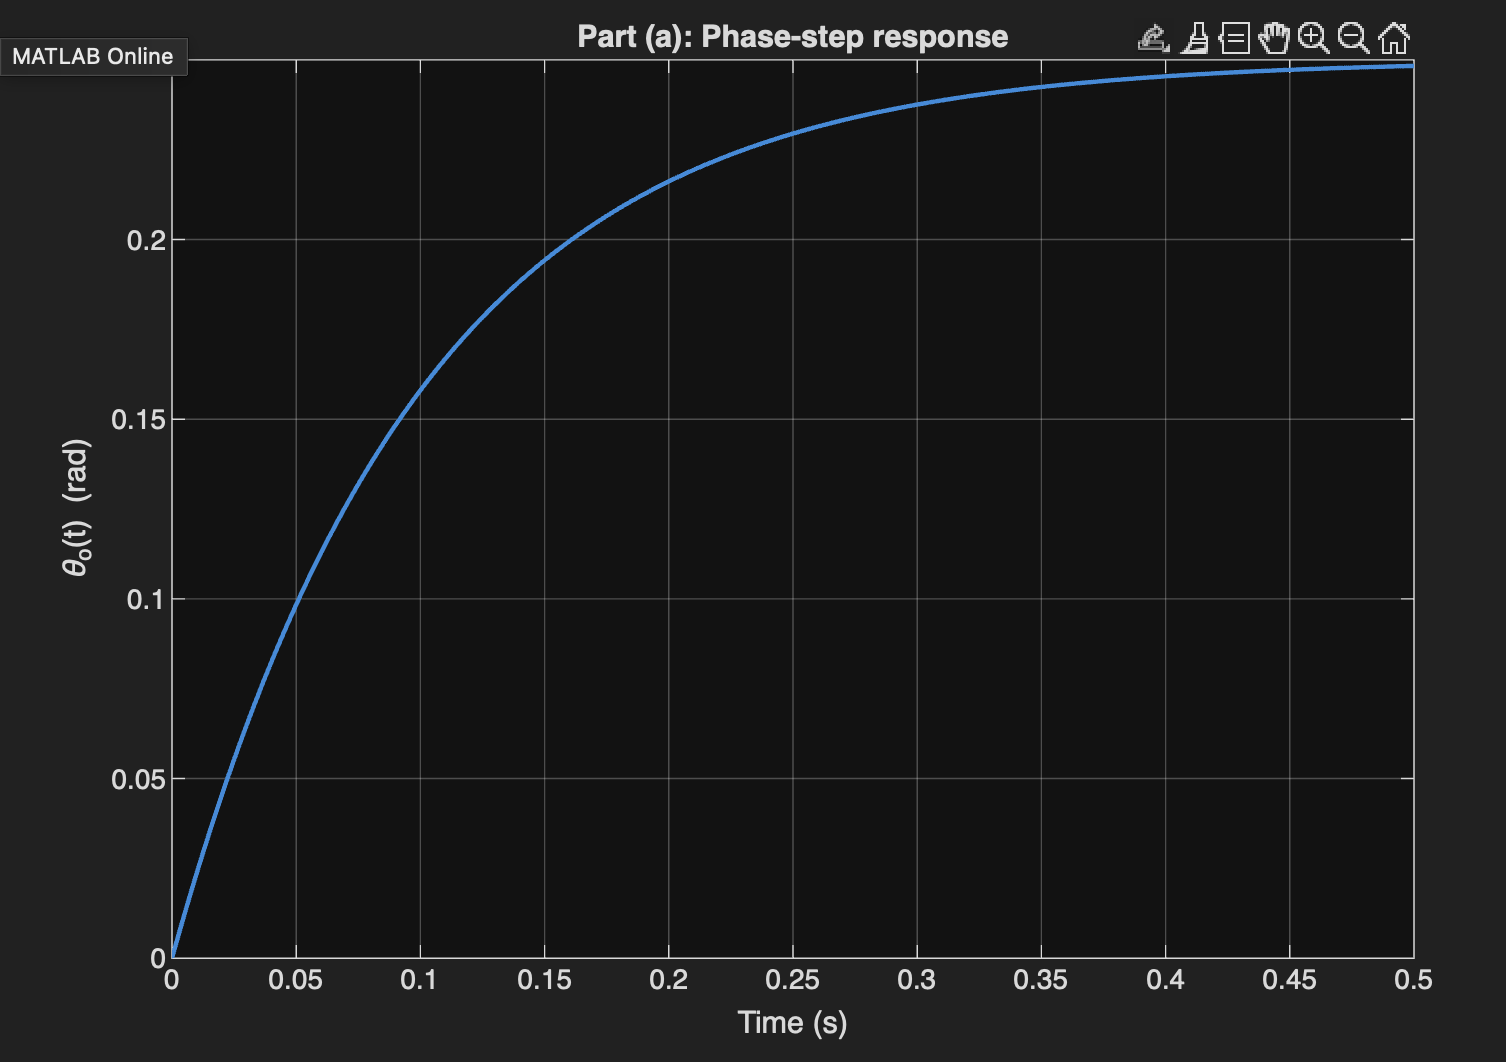
\includegraphics[width=0.75\linewidth]{question1a.png}
    \caption{Part (a) simulated phase-step response.}
  \end{figure}

  \item \(G(s)=1,\ \dot{\theta}_i(t)=2\pi k_f\,u(t)\Rightarrow \theta_i(t)=2\pi k_f\,t\,u(t)\).
  \[
    \Theta_i(s)=\frac{2\pi k_f}{s^2},\quad
    \Theta_o(s)=\frac{K}{s+K}\frac{2\pi k_f}{s^2}
    =\frac{2\pi k_f K}{s^2(s+K)} .
  \]
  Using \(d\theta_o/dt=\mathcal{L}^{-1}\{s\Theta_o(s)\}\),
  \[
    \frac{d\theta_o}{dt}=2\pi k_f\!\left(1-e^{-K t}\right),\qquad
    x(t)=\frac{2\pi k_f}{K_v}\left(1-e^{-K t}\right).
  \]
  The phase error is
  \[
    \theta_e(t)=\mathcal{L}^{-1}\!\left\{\frac{2\pi k_f}{s(s+K)}\right\}
    =\frac{2\pi k_f}{K}\left(1-e^{-K t}\right),
    \qquad \theta_e(\infty)=\frac{2\pi k_f}{K} \propto \frac{1}{K}.
  \]
  Larger loop gain \(K\) reduces the steady-state frequency-tracking error.
  \begin{figure}[h!]
    \centering
    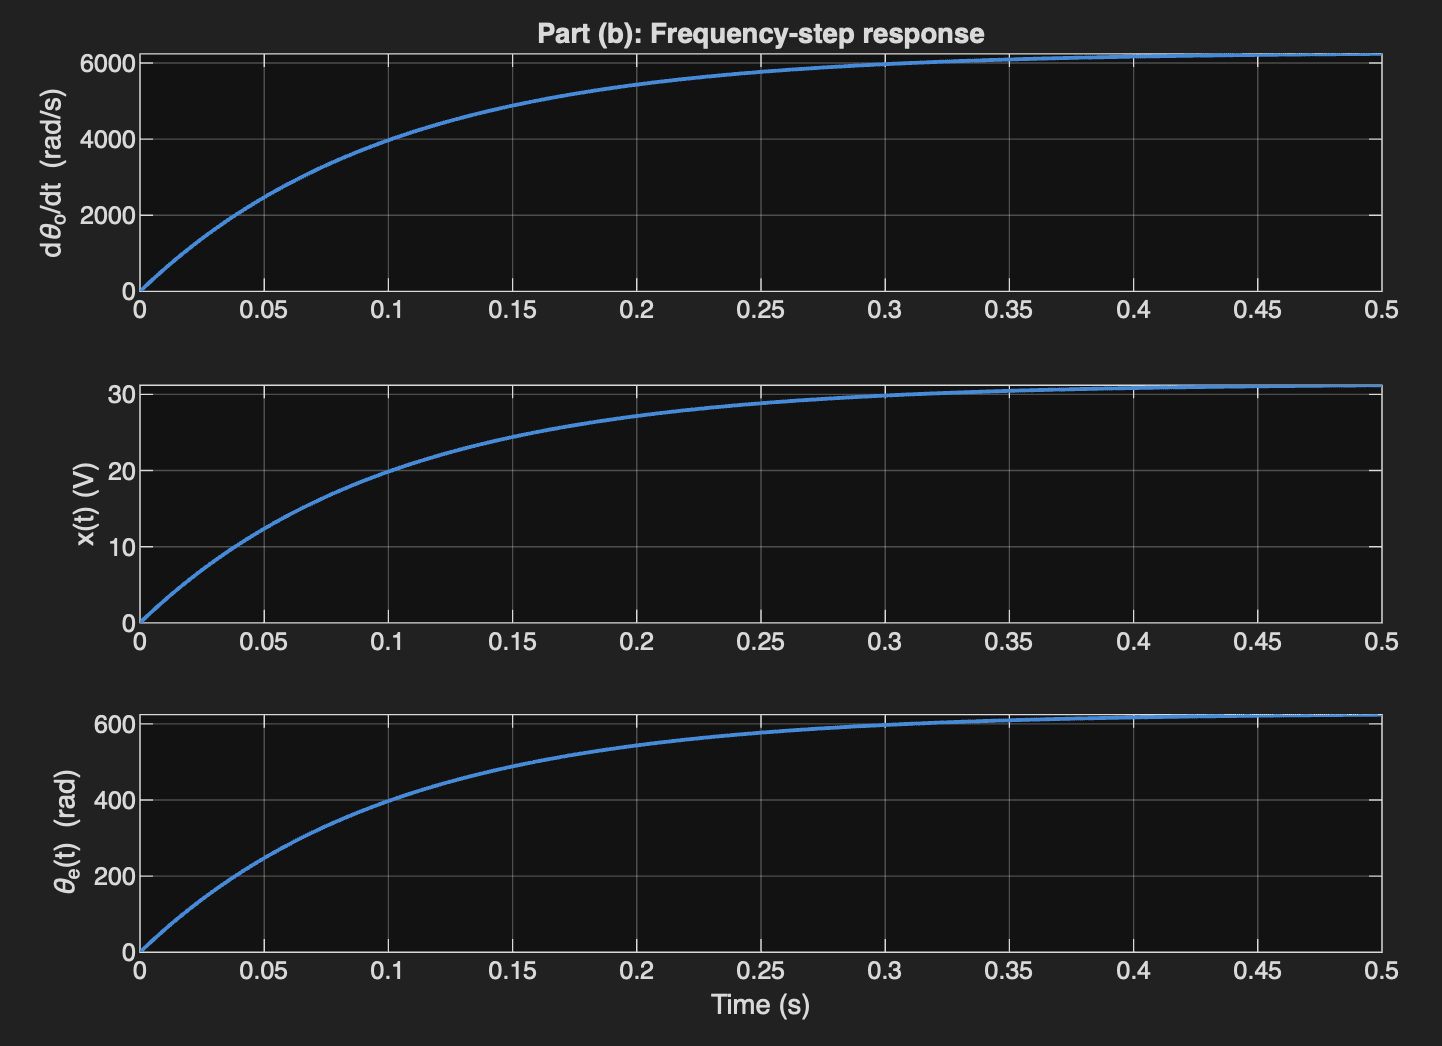
\includegraphics[width=0.9\linewidth]{question1b.png}
    \caption{Part (b) simulated frequency-step response (\(d\theta_o/dt\), \(x(t)\), and \(\theta_e(t)\)).}
  \end{figure}

  \item \(G(s)=\dfrac{s+a}{s},\ \dot{\theta}_i(t)=2\pi k_f\,u(t)\Rightarrow \Theta_i(s)=\dfrac{2\pi k_f}{s^2}\).
  \[
    H(s)=\frac{K(s+a)}{s^2+K(s+a)},\qquad
    \Theta_e(s)=\frac{2\pi k_f}{s^2+K(s+a)}.
  \]
  Steady-state values (final-value theorem):
  \[
    \theta_e(\infty)=\lim_{s\to 0} s\,\Theta_e(s)=0,
    \qquad
    x(\infty)=\lim_{s\to 0} s\,X(s)
    =\lim_{s\to 0}\frac{2\pi k_f K (s+a)}{K_v\,[s^2+K(s+a)]}
    =\frac{2\pi k_f}{K_v}.
  \]
  With the additional pole-zero in \(G(s)\), the loop becomes type-II and eliminates steady-state error to a frequency step.
\end{enumerate}

\end{document}
